\chapter{Tipos de processos de produção industrial}
\label{chap:tipos_de_processo_de_producao}

Nesta seção será discutida a classificação dos diversos tipos de empresas industriais partindo de seus processos de produção. Esta tarefa é importante na concepção de novas instalações industriais, pois permite identificar e reconhecer as características básicas da empresa industrial de acordo com o seu processo produtivo. 
Por fim, na seção \ref{sec:tipos_de_processo_de_producao_aplicacao} será mostrado a aplicação prática referente ao tipo de processo adotado pela \textit{SunBurn}.

\section{Sec1}
\label{sec:tipos_de_processo_de_producao_sec1}

As unidades produtivas podem variar desde o volume de produção (alto, médio ou baixo) até a variedade de seus produtos (alta, média ou baixa). Por isso, pode se dizer que as variáveis volume e variedade são dependentes entre si, por exemplo, operações de alto volume em geral têm baixa variedade de produtos e vice-versa. Portanto, existe uma relação inversa entre o volume e a variedade do produto \cite{slack2009administracao}.

A figura \ref{fig:tipos_de_processo_de_producao} nos mostra como os cinco tipos de processos existentes estão arranjados de acordo com o espectro variedade-volume. Além disso, as características de cada um destes processos serão descritos com base no volume e variedade, descendo pela diagonal que parte do canto superior esquerdo até canto inferior direito. Em outras palavras, os processos serão descritos a seguir partindo das empresas com uma maior variedade e baixo volume até uma empresa com baixa variedade e alto volume.

\begin{figure}[H]
  \caption{Matiz Variedade x Volume: Definindo os cinco tipos de processos produtivos ALTERAR A IMAGEM E O TITULO}
  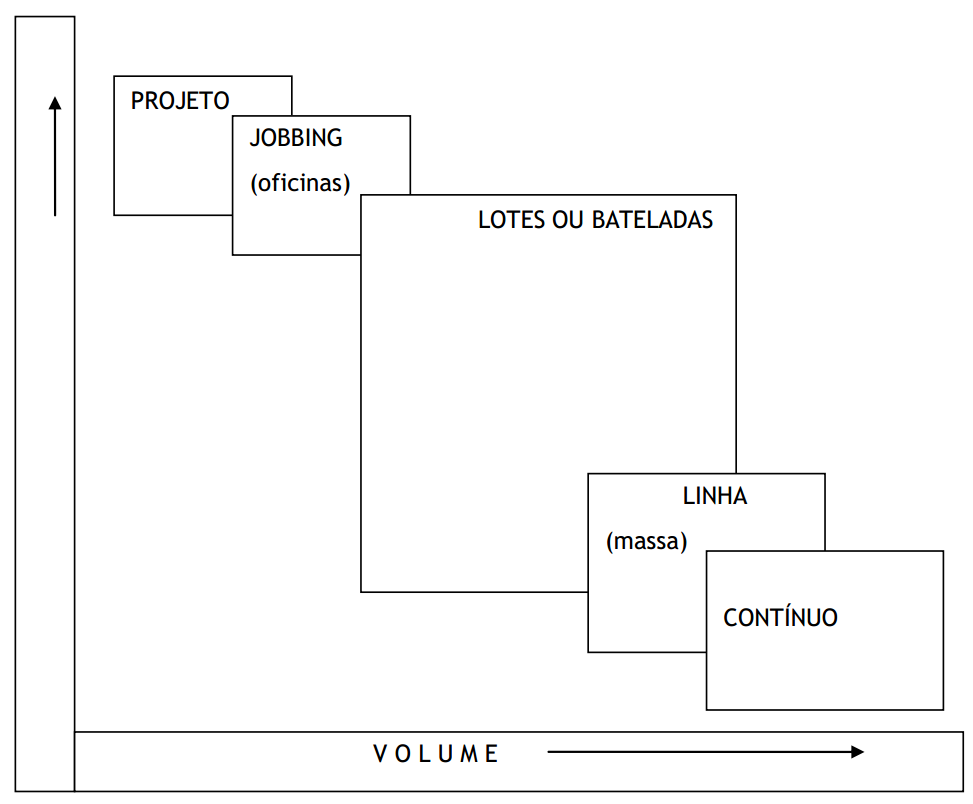
\includegraphics[scale=0.5]{images/tiposdeprocesso.png}
  \caption*{Fonte: Adptado de \cite{slack2009administracao}}
  \label{fig:tipos_de_processo_de_producao}
\end{figure}

O processo de projeto é caracterizado por possuir baixo volume, pois demora longos períodos para serem concluídos, e possuírem grande variedade entre os produtos entregues, como por exemplo, a construção de uma represa dificilmente haverá represas parecidas devido a questões geográficas de cada represa implantada.
\par O jobbing são também conhecido como oficinas pois possuem trabalhos feitos sob encomenda e por serem semi-artesanais. Um mesmo operador pode participar do processo de construção do produto do começo ao fim. Semelhante ao projeto, esse processo também possui grande variedade e baixo volume, e ao contrário deste não demora longos períodos para que o produto chegue na sua fase final, de entrega para o cliente. Um exemplo desse processo são as empresas de móveis planejados.
\par Já o processo por lotes ou bateladas, que é onde se encontra a maioria das empresas, é um estágio intermediário, das empresas que expandiram sua capacidade de produção (jobbing) mas ainda não se encontram no estágio de grandes unidades de produção automatizada. O termo lote refere-se a produtos contáveis, como por exemplo: bolas de futebol e lápis, já o termo batelada trata-se de produtos contínuos que para terem individualidade é necessário que sejam colocados em recipientes, como por exemplo: gasolina e leite. 
\par Os processos de produção em linha/massa possuem como característica principal a linha de fabricação/montagem, onde o produto percorre as várias estações de trabalho. Nesse tipo de processo tem-se um grande volume produzido e em contrapartida pouca variedade. Exemplo de fábrica que emprega este processo são as de fabricação de bicicletas.
\par E por último, no processo contínuo tem como característica serem quase sempre fluidos (gases, pastas, líquido e misturas) e que são processados no interior de tubulações e vasos fechados, além de possuírem elevada automação o que por sua vez acaba restringindo a quantidade de mão de obra operando as máquinas. Um exemplo deste processo são as refinarias de petróleo.


\section{Aplicação Prática}
\label{sec:tipos_de_processo_de_producao_aplicacao}

A SunBurn possui um processo com mínimas interrupções em todas as suas etapas e um grande volume produtivo. Estas características definem o processo como contínuo.    


